\documentclass[compress]{beamer}

\usetheme{Luebeck}
\usepackage[utf8]{inputenc}
\usepackage{subfig}
\usepackage{utopia} %font utopia imported
\usepackage{arabtex}
\usepackage{utf8}
\setcode{utf8}
\usepackage{amsmath}
\usepackage{amssymb}
\usepackage{amsthm}
\usefonttheme{professionalfonts} % using non standard fonts for beamer
\definecolor{foo}{RGB}{106,141,143}
\usecolortheme[named=foo]{structure}
\setbeamercolor{subsection in head/foot}{bg=foo!80!black}
% This block of code defines the information to appear in the
% title page

\title[ASIC Physical Design] %optional
{PowerPlanning}

\subtitle{How to Plan your own chip}

\author[Ahmed Abdelazeem] % (optional)
{Ahmed Abdelazeem}
%{A.~B.~Arthur\inst{1} \and J.~Doe\inst{2}}

\institute[ZU] % (optional)
{
	Faculty of Engineering\\
	Zagazig University
}
%{
	%	\inst{1}%
	%	Faculty of Engineering\\
	%	Zagazig University
	%	\and
	%	\inst{2}%
	%	Faculty of Chemistry\\
	%	Very Famous University
	%}

\date[ZU 2023] % (optional)
{RTL2GDSII Flow, February 2022}

%\logo{
\includegraphics[height=1.5cm]{lion-logo.png}}

%End of title page configuration block
%------------------------------------------------------------

%------------------------------------------------------------
%The next block of commands puts the table of contents at the
%beginning of each section and highlights the current section:
\setcounter{tocdepth}{1} %%%
\AtBeginSection[]
{
	\begin{frame}
		\frametitle{Table of Contents}
		\tableofcontents[currentsection]
	\end{frame}
}
%------------------------------------------------------------


\begin{document}
	
	%The next statement creates the title page.
	\frame{\titlepage}
	
	
	%---------------------------------------------------------
	%This block of code is for the table of contents after
	%the title page
	\begin{frame}
		\frametitle{Table of Contents}
		\tableofcontents
	\end{frame}
	%---------------------------------------------------------
%--------------------------------------------------
\section[Intro]{Introduction}
\subsection[Design]{PowerPlanning}
\begin{frame}
	\frametitle{PowerPlanning}
	\begin{center}
		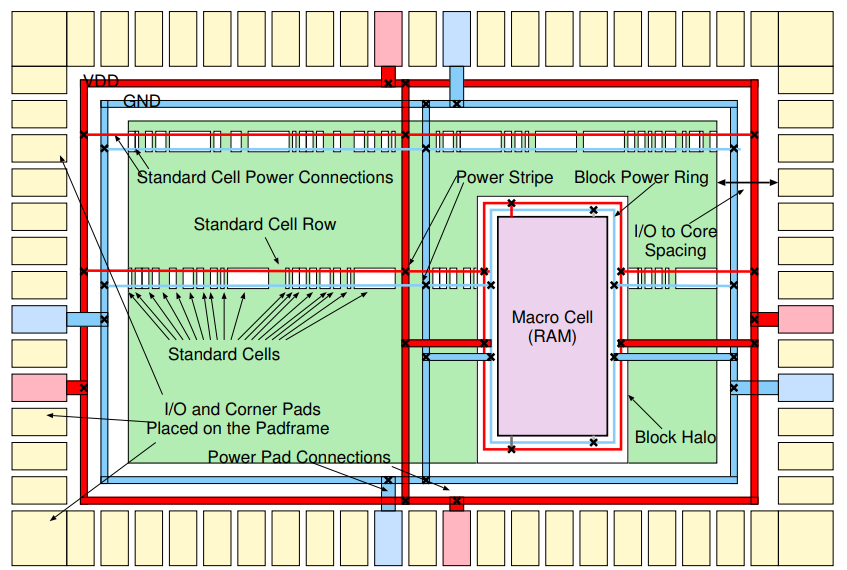
\includegraphics[width=\textwidth]{power}
	\end{center}
\end{frame}	
%-----------------------------------------------------
\subsection[Objective]{Objective of PowerPlanning}
\begin{frame}
	\frametitle{Objective of PowerPlanning}
	\begin{itemize}
		\item To distribute the power from power pads to all elements in the chip.
		\item Unified supply of power with less voltage drop
		\item A proper Power design should aim at using as less routing recourse as possible.
		\item Power Analysis (EMIR) check should be done after power planning is completed 
	\end{itemize}
\end{frame}

\subsection[Power]{PowerPlanning}
\begin{frame}
	\frametitle{PowerPlanning}
	\begin{itemize}
		\item Creation of the power network within a design
		\item Power planning is integrated with the overall design flow and must be taken into account early in the design process because: 
			\begin{itemize}
				\item \# of pads may determine physical size (pad limited). 
				\item The power structures within the core area consume physical area.
				\item The power grid topology effects top level routability, and also placement and routing within the child blocks.
				\item The power structure effects functionality and reliability.
			\end{itemize}
	\end{itemize}
\end{frame}

\begin{frame}
	\frametitle{Simplified Power Distribution Architecture}
	\begin{center}
		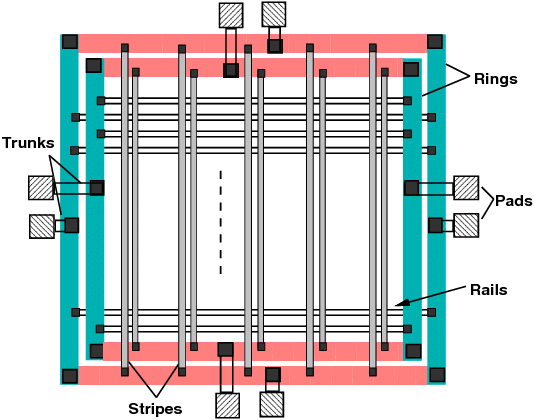
\includegraphics[width=0.8\textwidth]{Power-Ground-Distribution-Network}
	\end{center}
\end{frame}

\begin{frame}
	\frametitle{Power Network Elements }
	\begin{itemize}
		\item \textbf{Power Pad} 
		\item \textbf{Trunks}
			\begin{itemize}
				\item Connects Ring to Power Pad
			\end{itemize}
		\item \textbf{Power Rings}
			\begin{itemize}
				\item Form complete rings around the periphery of the die, around individual hard macros, or inside of hierarchical blocks
				\item higher-level Metal layers Power
			\end{itemize}			
		\item \textbf{Power Stripes}
			\begin{itemize}
				\item Carries VDD and VSS from Rings across the chip
				\item Horizontal and vertical metal wires placed in an array across the entire or section die
				\item higher level routing layers \item typically uniformly distributed across the die.
			\end{itemize}
		\item \textbf{Power Rails}
			\begin{itemize}
				\item Is used to connect the standard cell power rails together, and or power straps.
				\item Low level, typically metal 1.
			\end{itemize}
	\end{itemize}
\end{frame}

\begin{frame}
	\frametitle{Power Estimations}
	Power Estimation is based on total power consumed by the chip:
		\begin{itemize}
			\item IO Power
			\item Core Power (Std. Cells +Macros)
		\end{itemize}
		\begin{center}
			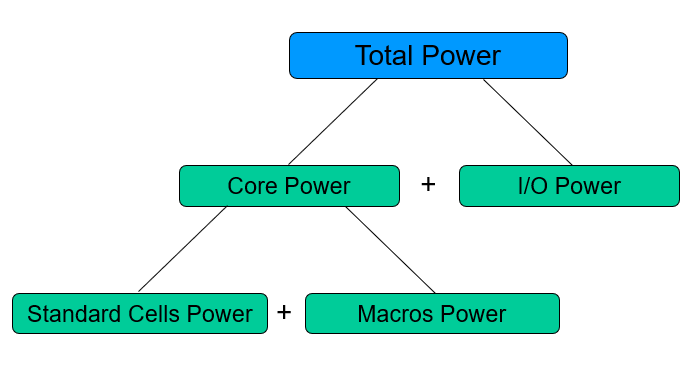
\includegraphics[width=\textwidth]{power2}
		\end{center}
\end{frame}

\begin{frame}
	\frametitle{Power Planning}
		\begin{itemize}
			\item Power Planning includes: 
			\begin{itemize}
				\item proper Estimation of power of chip
				\item power routing the design based on the estimation.
			\end{itemize}
			\item We create a mesh kind of structure, so that instance(s)
			can take direct supply from the nearest point
			\item We create multiple VDD and VSS lines(for each
			power domain)
			\item Hierarchical Mesh from upper metal layers to
			lowest(Ml or M2 layers for standard cells). Connection
			from higher to adjacent lower metal layer is through
			VIAs
		\end{itemize}
\end{frame}
\begin{frame}
	\frametitle{Power Mesh}
\begin{itemize}
	\item Power/Ground mesh will allow multiple paths
	from P/G sources to destinations		
	\begin{itemize}
		\item Hierarchical power and ground meshes
		from upper metal layers to lower metal layers
		\item  Multiple vias between layers
	\end{itemize}
\end{itemize}

	\begin{center}
		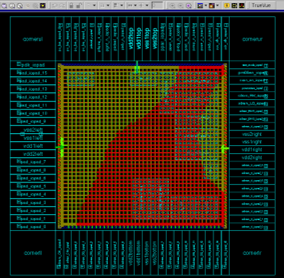
\includegraphics[width=0.4\textwidth]{Power mesh}
	\end{center}
\end{frame}
\begin{frame}
	\frametitle{Why create mesh kind of structure ?}
	\begin{itemize}
		\item  To distribute the Power from power pads/pins to all elements of the chip.
		\item Provides multiple paths from PG sources to destinations (less series resistance)
		\item  Uniformly distribute power with less voltage drop.
		\item  To meet IR/EM targets
		\item  For meeting timing requirements
	\end{itemize}
	\begin{center}
	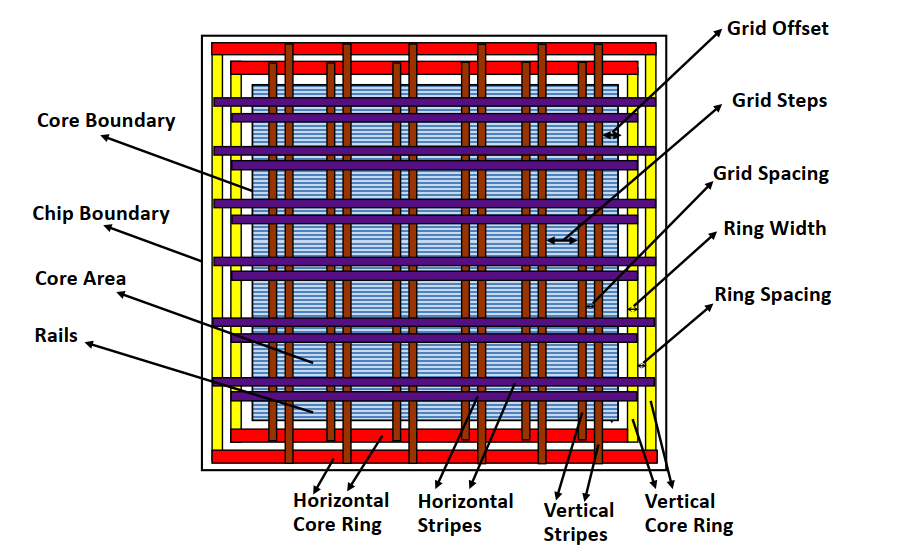
\includegraphics[width=0.5\textwidth]{Power mesh2}
\end{center}
\end{frame}
\begin{frame}
	\frametitle{Power Planning vs. Power Routing}
	\begin{center}
		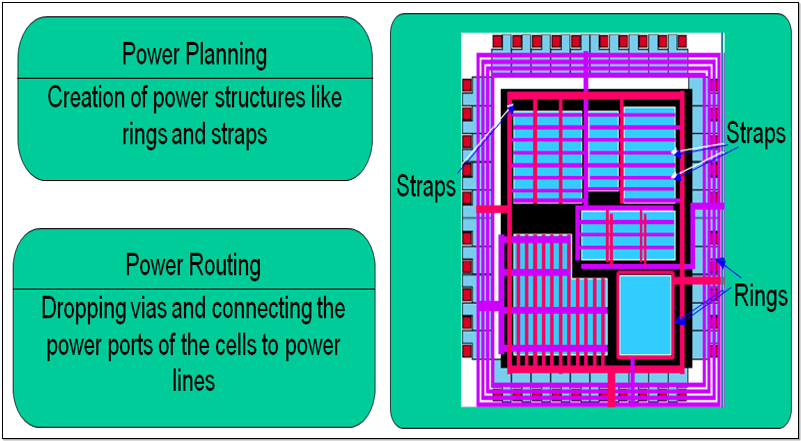
\includegraphics[width=\textwidth]{Power Planning vs. Power Routing}
	\end{center}
\end{frame}
%-------------------------------------------------
\section[Issues]{Power Planning Issues}
	\subsection[IR Drop]{IR Drop}
	\begin{frame}
		\frametitle{IR Drop}
		\begin{itemize}
			\item Reduction in voltage that occurs on power supply networks
			\item IC design expects availability of ideal power supply
			\item In reality, localized voltage drops within the power grid
		\begin{itemize}
			\item Increasing current/area on die
			\item Narrower metal line widths (increases power grid resistance)
		\end{itemize}
			\item Results in decreased power supply voltage at cells/transistors
			\item Decreases the operating voltage of the chip, resulting in timing and functional failures
		\end{itemize}
	\begin{center}
		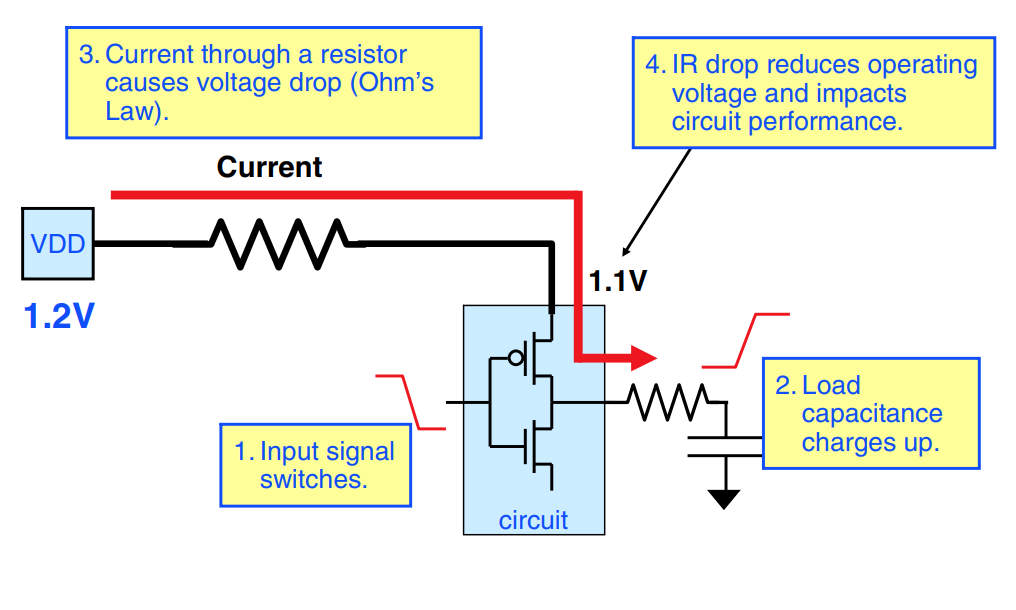
\includegraphics[width=0.5\textwidth]{IR4}
	\end{center}
	\end{frame}
\begin{frame}
	\frametitle{Reasons of IR Drop Violations}
	\begin{itemize}
		\item Power structure is not proper.
		\item Cell density is very high.
		\item Instances are not get proper power because of no straps
		over there
		\item Mesh structure is proper but there is no via
	\end{itemize}
\end{frame}
\begin{frame}
	\frametitle{How to reduce IR drop ?}
	\begin{itemize}
		\item Routing should be from Top Layer.
		\item By adding some more Power Stripes.
		\item By increasing the width of the metal.
		\item By adding Decaps(DCAP cells).
		\item By using some Low Power Techniques
	\end{itemize}
\end{frame}
%-----------------------------------------------------
\subsection[Ground Bounce]{Ground Bounce}
\begin{frame}
	\frametitle{Ground Bounce}
	\begin{itemize}
		\item Increase in voltage that occurs on ground networks (VSS or GND) in integrated circuits
		\item Increase in ground voltage decreases the operating voltage of the chip, resulting in timing and
		functional problems
	\end{itemize}
	\begin{center}
		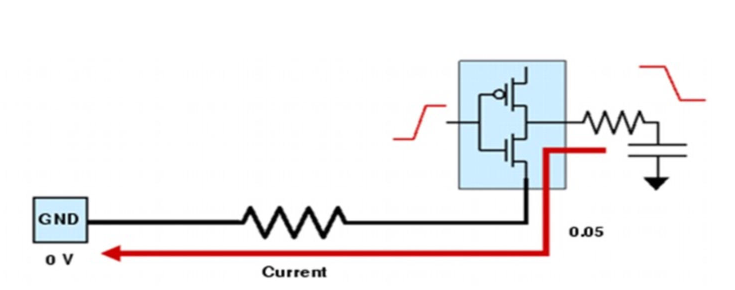
\includegraphics[width=0.7\textwidth]{ground}
	\end{center}
\end{frame}
%---------------------------------------------------
\subsection[EM]{EM violations}
\begin{frame}
	\frametitle{Electromigration}
		\begin{itemize}
			\item  Electromigration is the movement of atoms based on the flow of current through a material. 
			\item If the current density is high enough, the heat dissipated within the material will repeatedly break atoms from the structure and move them.
			\item Results of EM in ICs: The \textcolor{red}{VOIDs} and \textcolor{red}{HILLOCKS} gets created and potentially
			causing open and short circuits.
		\end{itemize}
	\begin{center}
		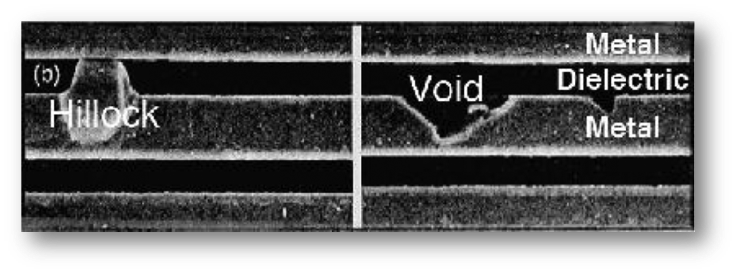
\includegraphics[width=\textwidth]{EM}
	\end{center}
\end{frame}
\begin{frame}
	\frametitle{EM violations : Reasons of EM violation}
	\begin{itemize}
		\item High Fanout Net (multiple fanout cells switch simultaneously, draws larger
		current from driver)
		\item Higher Driver Strength Cells(delivers large current unnecessarily, heating up the wire)
		\item Higher frequency(quick transitions)
		\item Narrow metal width
		\item Metal slotting (resulting into narrower widths)
		\item Long Nets (because of larger resistance, higher localized temperature)
	\end{itemize}
\end{frame}
\begin{frame}
	\frametitle{Solutions of EM violations}
	\begin{itemize}
		\item Decrease Driver’s drive Strength.
		\item NonDefault (wider) rule based routing.
		\item Insert buffer on long nets.
		\item Route with higher metal layers(lessresistive, higher tolerance (current carrying capabilities)
		\item Use multi-Cut Via
		\item Break the fanout (have lesser fanouts)
		\item Use wider metals (more width)
	\end{itemize}
\end{frame}
%---------------------------------------------------
\section[Checks]{Power Plan Checks}
\subsection[Checks]{Power Plan Checks}
\begin{frame}
	\frametitle{Power Plan Checks}
	\begin{itemize}
		\item There should be no open connection
		\item All the Macros should be hooked up with Power/Ground.
		\item IR/EM target should be met.
		\item Missing Vias should be taken care
		\item There should be no Hot Spots (during IR-Drop Analysis)
	\end{itemize}
\end{frame}
%---------------------------------------------------	
\begin{frame}
	\frametitle{....}
	\begin{center}
		\<بِسْمِ اللَّـهِ الرَّحْمَـٰنِ الرَّحِيمِ> \\
		\<وَمَا أُوتِيتُمْ مِنَ الْعِلْمِ إِلَّا قَلِيلً>
		
	\end{center}
\end{frame}
%---------------------------------------------	
\end{document}	